\documentclass[]{beamer}
\usepackage[T1]{fontenc}
\usepackage[utf8]{inputenc}
\usepackage{lmodern}
\usepackage[italian]{babel}

\title{Informatica per l'azienda}
\author{Mattia Cozzi}
\date{a.f.~2024/2025}


%\documentclass[handout]{beamer}     %usare questa classe per generare l'handout

%\usepackage{pdfpages}   %per mostrare più quadri nella stessa pagina
%\pgfpagesuselayout{4 on 1}[a4paper,border shrink=5mm,landscape]


\usetheme{Singapore}
%\useoutertheme[left]{sidebar} %elementi intorno alle diapositive
\setbeamercovered{dynamic} %modifica l'aspetto del testo grigetto delle diapositive future. Argomenti: invisible/transparent/dynamic


%COLORE PRINCIPALE
\definecolor{verde}{RGB}{2, 194, 117} % UBC Blue (primary)
\setbeamercolor{structure}{fg=verde} % itemize, enumerate, etc
\setbeamercolor{alerted text}{fg=verde}


\usecolortheme{orchid}

\usepackage{tikz}

\begin{document}

\begin{frame}
  \titlepage
\end{frame}


\begin{frame}
\frametitle{Contenuti}
\tableofcontents
\end{frame}



\section{Sistemi informativi}


\begin{frame}
\frametitle{Il ``sistema impresa''}
Il ``sistema impresa'' è composto da parti interdipendenti e correlate:
\begin{itemize}
  \item sistema decisionale;
  \item sistema organizzativo;
  \item sistema di controllo;
  \item \alert<1>{sistema informativo}.\pause
\end{itemize}

~

Il sistema informativo aziendale consiste nell'insieme di flussi di conoscenza (dati e informazioni) ricorrenti e individuabili nell'organizzazione, in forma sia cartacea sia digitale.
\end{frame}



\begin{frame}
\frametitle{Sistema informativo aziendale}
Un SIA si occupa ad esempio di gestire le informazioni relative a:
\begin{columns}
\begin{column}{.4\textwidth}
  \begin{itemize}
    \item contabilità;
    \item magazzino;
    \item marketing;
  \end{itemize}
\end{column}
\begin{column}{.4\textwidth}
  \begin{itemize}
    \item posta elettronica;
    \item gestione clienti.
  \end{itemize}

  ~
\end{column}
\end{columns}
\pause

~

~

In generale, un sistema informativo si occupa di acquisizione, elaborazione, archiviazione, trasmissione e presentazione dei dati.\pause

~

Chiaramente, \alert<3>{l'informazione riveste un ruolo chiave all'interno dell'organizzazione aziendale} (si pensi al processo decisionale) e la sua gestione è affidata all'\alert<3>{informatica}.
\end{frame}



\begin{frame}
\frametitle{Sistema informatico}
Il sistema informatico è la \alert<1>{porzione informatizzata del sistema informativo}, composto da strumenti hardware e software che gestiscono i flussi di informazioni.\pause

~

Nel mondo contemporaneo la globalizzazione, la trasformazione delle imprese e dell'economia stessa hanno permesso la nascita di nuove soluzioni software dette ERP, acronimo di \alert<2>{Enterprise Resource Planning}.\pause

~

Questi servizi propongono un sistema integrato di gestione delle informazioni mediante moduli software che operano su un'unica base di dati opportunamente concepita.
\end{frame}




\section{ERP}

\begin{frame}
\frametitle{Enterprise Resource Planning}
I \alert<1>{sistemi informativi integrati}, o ERP, rappresentano un'evoluzione dei sistemi informativi aziendali.\pause

~

Le applicazioni ERP consentono una completa integrazione dei processi d'impresa, offrendo gli strumenti per una gestione unitaria dell'azienda. Un ERP ha moduli per:
\begin{itemize}
  \item gestione fornitori;
  \item gestione rete di vendita;
  \item gestione clienti.
  \item gestione magazzino;
  \item gestione contabilità.
\end{itemize}\pause

~

In generale, un sistema ERP è una \alert<3>{architettura software} che facilita il flusso di informazioni tra le funzioni interne dell'azienda. Le informazioni sono contenute e organizzate in un \alert<3>{database aziendale}.
\end{frame}




\begin{frame}
\frametitle{Caratteristiche dei sistemi ERP}
\begin{description}
  \item[Unicità della base di dati] Garantisce la tracciabilità e la veridicità dei dati, evitando inoltre la ridondanza dei dati. Permette di avere sempre informazioni condivise e aggiornate.\pause
  
  ~

  \item[Configurabilità del sistema] I sistemi ERP sono molto flessibili, perché aziende diverse hanno metodi operativi ed esigenze diversi. Permettono inoltre l'integrazione con procedure già esistenti in azienda.\pause
  
  ~
  
  \item[Modularità del sistema] Essendo composti da moduli separati, è possibile un passaggio graduale all'utilizzo del nuovo sistema. Questa struttura rende anche più agevole la manutenzione del sistema stesso· 
\end{description}
\end{frame}


\begin{frame}
\frametitle{Moduli di un sistema ERP}
\begin{itemize}
  \item Contabilità
  \item Controllo di gestione
  \item Gestione del personale
  \item Gestione degli acquisti
  \item Gestione dei magazzini
  \item Gestione della produzione
  \item Gestione dei progetti
  \item Gestione delle vendite
  \item Gestione della distribuzione
  \item Gestione degli asset
\end{itemize}
\end{frame}



\begin{frame}
\frametitle{Software ERP sul mercato}
A pagamento, dietro pagamento di licenza:
\begin{itemize}
  \item Microsoft Dynamics;
  \item SAP.
\end{itemize}\pause

~

Open source:
\begin{itemize}
  \item ERPNext;
  \item OpenERP;
  \item openbravo.
\end{itemize}
\end{frame}





\begin{frame}
\frametitle{Fatturazione elettronica}
Nel 2015 è divenuto obbligatorio per le aziende regolare i propri rapporti commerciali con la PA attraverso la fattura elettronica per la cessione di beni o servizi effettuati. È un sistema efficiente, veloce, sicuro ed economico.\pause

~

Il nuovo documento:
\begin{itemize}
  \item è un file XML (\emph{eXtensible Markup Language}) che viene prodotto dal fornitore;\pause
  \item riceve una formattazione particolare definita dalla PA;\pause
  \item viene sottoscritto con firma elettronica;\pause
  \item viene spedito mediante PEC.
\end{itemize}
\end{frame}

\begin{frame}
\frametitle{Esempio di file XML}
\begin{figure}
  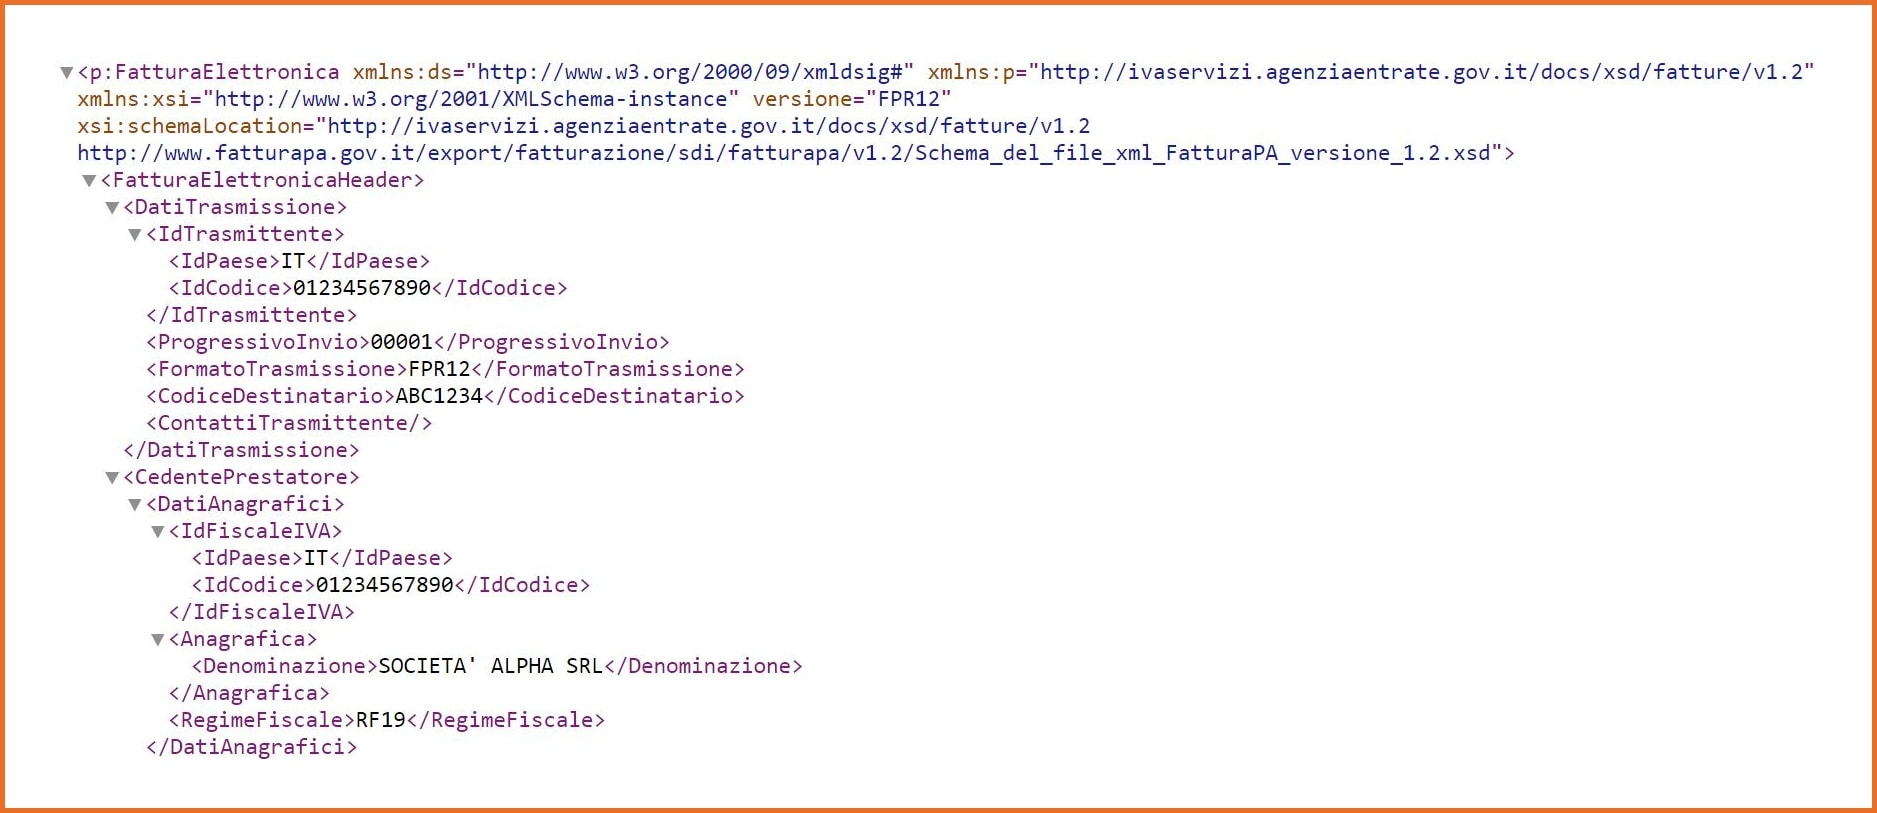
\includegraphics[width=\columnwidth]{img/xmlfattura.jpg}
\end{figure}
Il file XML viene poi formattato e visualizzato in PDF.
\begin{center}
  \href{https://www.fatturapa.gov.it/it/lafatturapa/esempi/}{\beamergotobutton{Esempi forniti dalla PA}}
\end{center}
\end{frame}

\section{Glossario}

\begin{frame}
\frametitle{Glossario}
\begin{itemize}
  \item \alert{Anagrafica:} insieme ordinato di informazioni che permettono di identificare e descrivere un operatore o un'azienda. La legge stabilisce che le aziende devono conservare una scheda anagrafica per ogni cliente e fornitore.
  
  ~
  
  \begin{figure}
    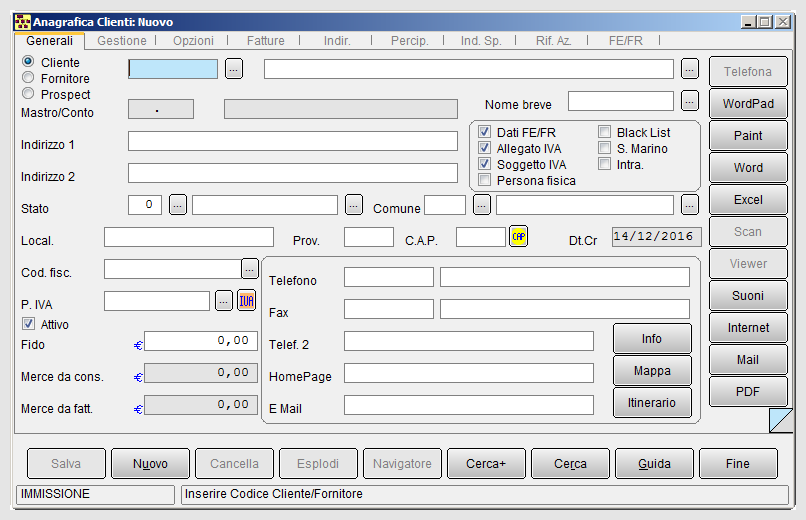
\includegraphics[width=.6\columnwidth]{img/anagrafica.png}
  \end{figure}
\end{itemize}
\end{frame}

\begin{frame}
\frametitle{Glossario}
\begin{columns}
  \begin{column}{.55\textwidth}
    \begin{itemize}
      \item \alert{Documento di trasporto (DDT):}  è un documento previsto dalla legge italiana, precedentemente noto come ``bolla di accompagnamento''. Con l'introduzione di un sistema gestionale informatico, il DDT è uno dei primi documenti (insieme alla fattura, e agli ordini) a essere configurati e implementati.
    \end{itemize}
  \end{column}
  \begin{column}{.5\textwidth}
    \begin{figure}
      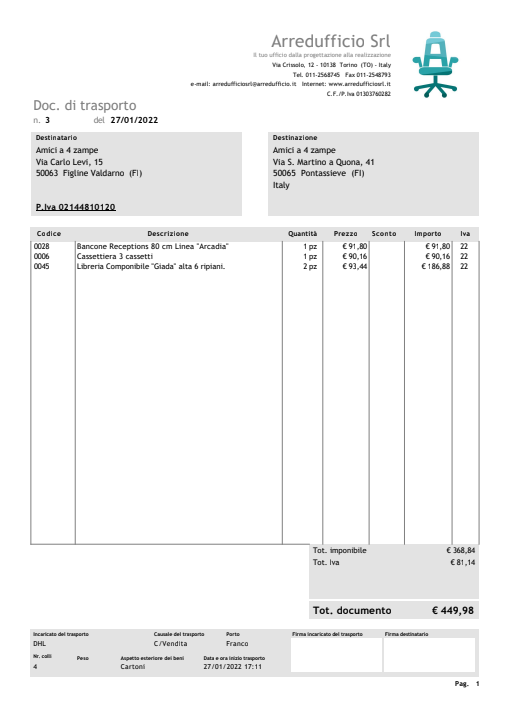
\includegraphics[width=\columnwidth]{img/ddt.png}
    \end{figure}
  \end{column}
\end{columns}
\end{frame}

\begin{frame}
\frametitle{Glossario}
\begin{columns}
  \begin{column}{.55\textwidth}
    \begin{itemize}
      \item \alert{Fattura:} è un documento emesso dai soggetti con Partita Iva che comprova la vendita di una merce o la prestazione di un servizio. I software di ERP hanno procedure automatiche per emettere fatture, ma richiedono che i dati di partenza inseriti dagli operatori siano precisi e completi.
    \end{itemize}
  \end{column}
  \begin{column}{.5\textwidth}
    \begin{figure}
      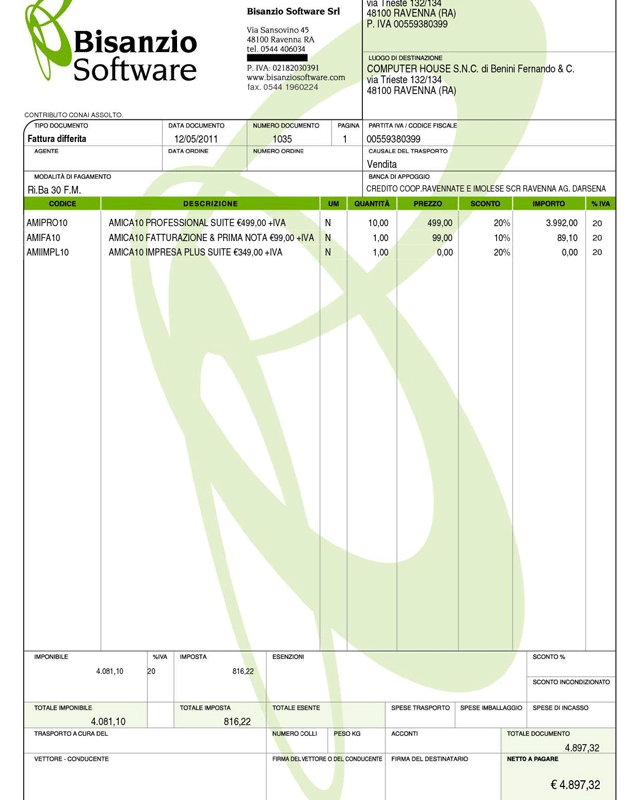
\includegraphics[width=\columnwidth]{img/fattura.png}
    \end{figure}
  \end{column}
\end{columns}
\end{frame}



\begin{frame}
\frametitle{Glossario}
\begin{itemize}
  \item \alert{Libro giornale:} registro contabile in cui vengono registrati giorno per giorno tutti i movimenti di una determinata azienda, in un dato periodo di tempo. Il libro giornale è tenuto con il metodo della partita doppia. Le operazioni segnate hanno il nome di articoli.
  
  ~

  \begin{figure}
    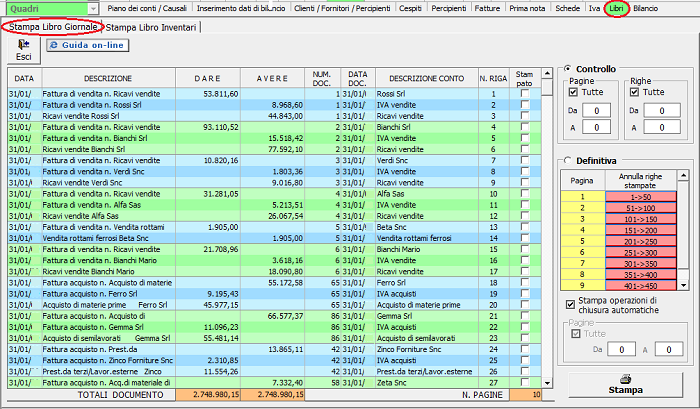
\includegraphics[width=.7\columnwidth]{img/librogiornale.png}
  \end{figure}
\end{itemize}
\end{frame}



\begin{frame}
\frametitle{Glossario}
\begin{itemize}
  \item \alert{Database:} raccolta di dati progettati in modo tale da poter essere utilizzati in maniera ottimizzata da diverse applicazioni e diversi utenti. La caratteristica principale dei database è di avere dati collegati tra loro mediante uno schema che l'utente può comprendere e navigare. I dati possono anche essere estratti per essere stampati.  
  \begin{figure}
    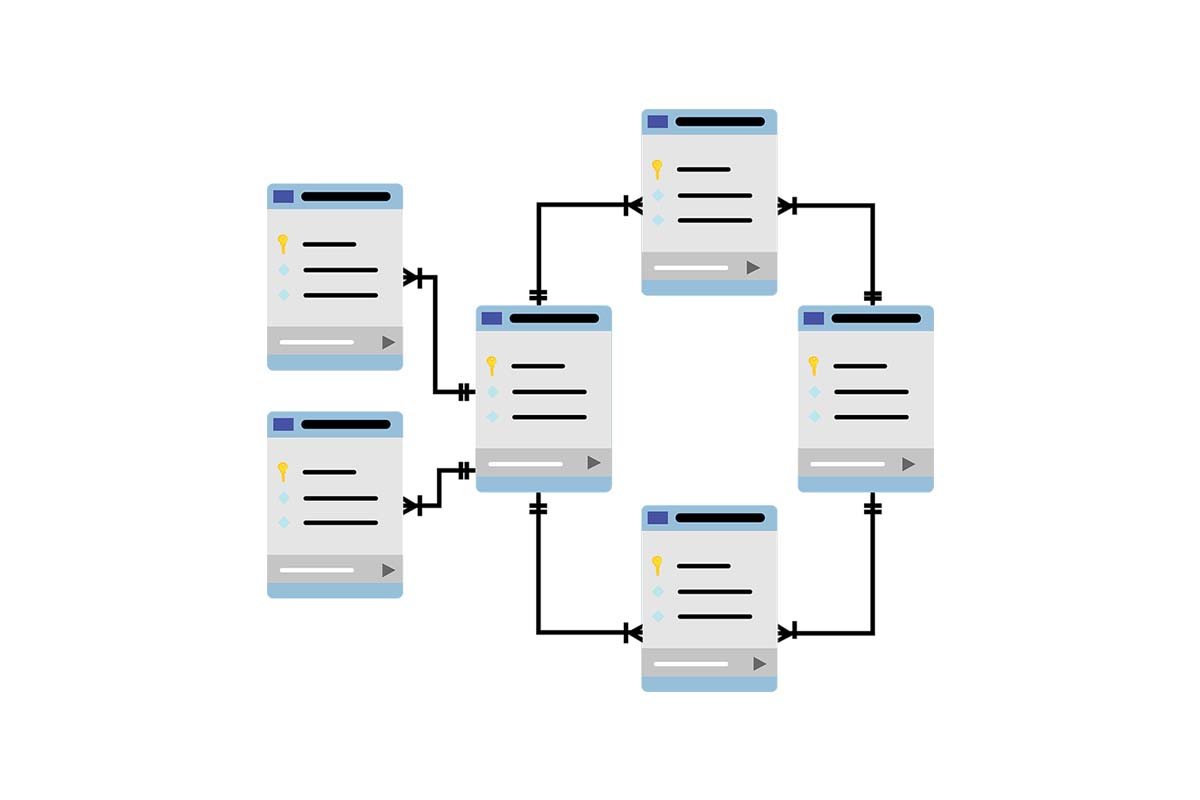
\includegraphics[width=.7\columnwidth]{img/database.jpg}
  \end{figure}
\end{itemize}
\end{frame}



\begin{frame}
\frametitle{Glossario}
\begin{itemize} 
  \item \alert{Cespite (\emph{asset}):} è un bene materiale o immateriale acquistato dall'azienda e che ha un ciclo di vita superiore ad un anno. Esempi di cespiti materiali sono gli edifici, i capannoni, le strumentazioni, i macchinari, i computer, eccetera. Esempi di cespiti immateriali sono i brevetti, le concessioni di licenze e marchi, i costi di ricerca e sviluppo, eccetera.
  
  ~
  
  \begin{columns}
    \begin{column}{.4\textwidth}
      \begin{figure}
        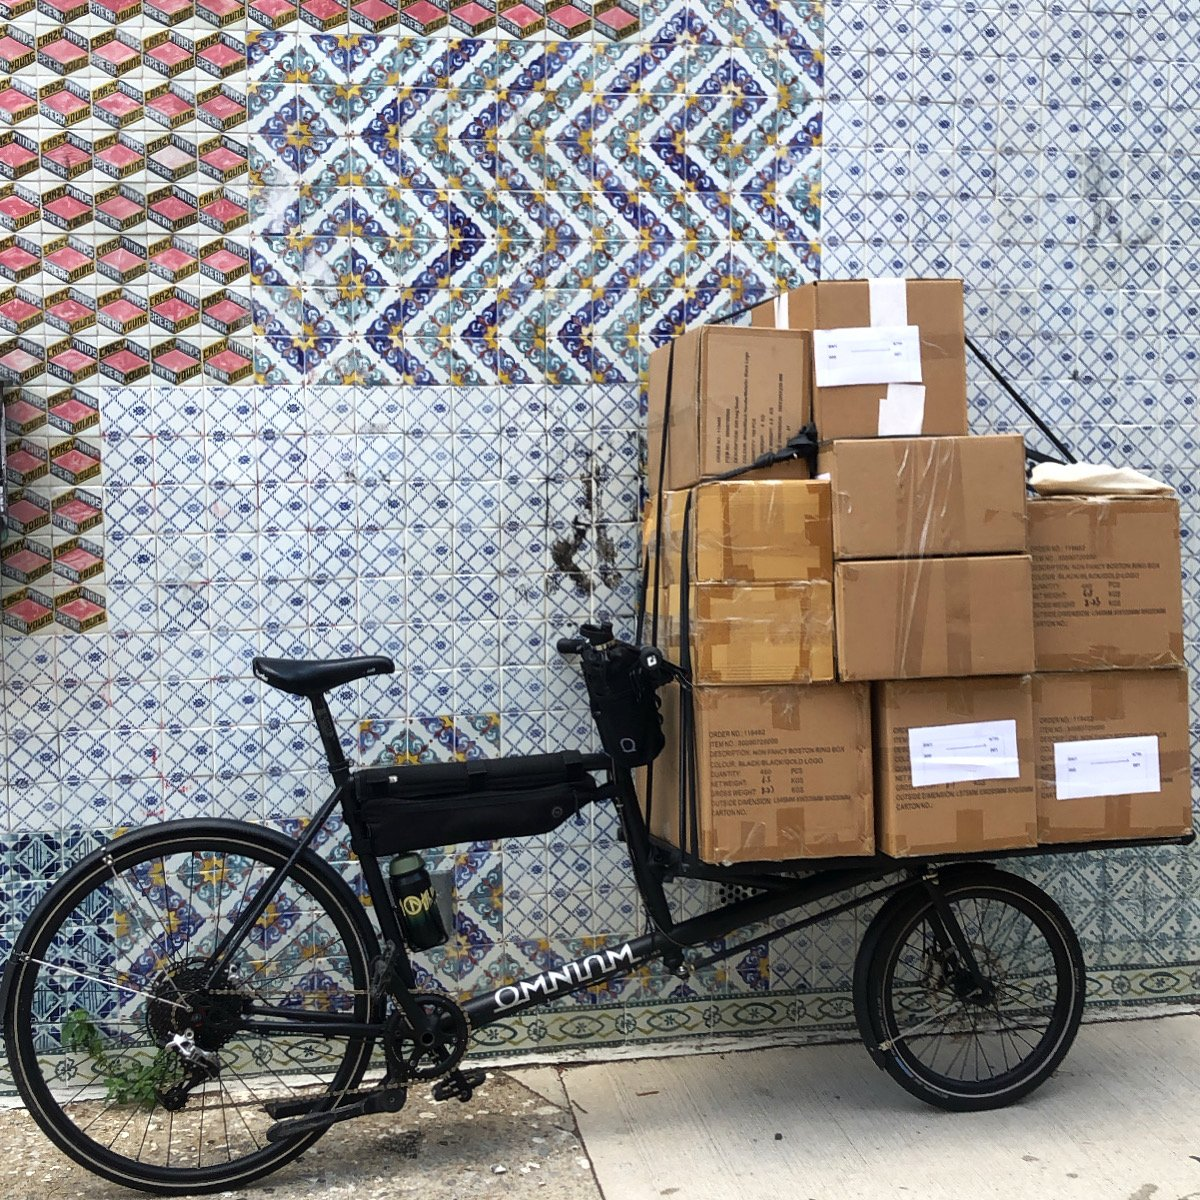
\includegraphics[width=\columnwidth]{img/cargobike.jpg}
      \end{figure}
    \end{column}
    \begin{column}{.4\textwidth}
      \begin{figure}
        
\includegraphics[width=\columnwidth]{img/g1.jpg}
      \end{figure}
    \end{column}
  \end{columns}
\end{itemize}
\end{frame}

\end{document}
